\section{Braking}
The brake system in a vehicle is undeniably one of its most critical components, serving the vital function of controlling its speed and ensuring safe stops when necessary.


\subsection{Overview}
With various types of braking systems available:

\begin{itemize}
    \item Mechanical Brake System
    \item Hydraulic Brake System
    \item Pneumatic Brake System
    \item Electromagnetic Brake System
    \item Electrical Brake System
    
\end{itemize}

Among these options, we have opted to implement the pneumatic braking system due to its simplicity in construction and its ability to provide a fail-safe mechanism through selection types. Pneumatic brakes offer reliable performance and can be well-suited for various vehicle applications, particularly those requiring robust and efficient braking capabilities.
\subsubsection{Requirements and Constraints}
In designing and implementing a vehicle's braking system or pod, careful attention is put on specific requirements and considerations. The complex design for the braking system of a pod depends largely on the maximum speed that can be achieved by the vehicle. Faster speeds call for finer brake parts to allow for proper and safe deceleration hence putting more emphasis on exactness in the system design. On top of this, knowing how much energy that is stored in it is vital to ensure safe braking operations. It is therefore important to discharge this energy properly during braking so as to avoid overheating, mechanical failure, and to preserve the reliability of this system.\\


Moreover, there are certain restrictions to be followed in order for the braking process to be effective. These also include handling efficiently static weight of the pod plus any additional loads experienced during operation. Also, it should be designed with respect to high vehicle speed when considering stopping power within a reasonable range for safety purposes of passengers. Knowledge about distance required stopping is very significant here; such that brakes are made so as they can safely cause deceleration within that distance hence preventing accidents from happening.By adhering meticulously to these requirements and constraints, a braking system can be designed and implemented effectively, ensuring the safety and optimal performance of the pod.

\subsubsection{Concept}
Our major objective is simple: to develop a brake system that can never fail, guaranteeing the highest level of dependability and safety. Important components of the system include actuators, springs, and a pneumatic system. The pre-compressed springs provide the majority of the braking force, while the pneumatic system and actuators help in controlling and holding them in position.
Because a pneumatic system reacts rapidly, which is essential for effective braking, we decided to retract the spring using it. Although we might think about utilizing electrical actuators, their cost is prohibitive and would necessitate a large budget adjustment for the entire pod. For the purposes of our project, the pneumatic technique makes the most sense.





\section{Size, Components, and Appearance}

\begin{table}[htbp]
\centering
\begin{adjustbox}{width=\textwidth} % Adjust table width to fit textwidth
\begin{tabular}{|c|c|c|c|c|c|}
\hline
\textbf{Component} & \textbf{Number} & \textbf{Mass [g]} & \textbf{Size [mm]} & \textbf{Material} & \textbf{In-house/Outsourced} \\
\hline
\textbf{Main Spring} & $\times$16 & 3163.2 & - & - & - \\
\textbf{Brake Pad} &$\times$16 & 406.4 & - & - & - \\
\textbf{Pad Mounting Bracket} & $\times$4 & 2296.6 & - & - & - \\
\textbf{Big Actuator} & $\times$4 & 8868 & - & - & - \\
\textbf{Small Actuator} &$\times$8 & 2432 & - & - & - \\
\textbf{Tube 8mm} & $\times$5 & - & - & - & - \\
\textbf{Tube 6mm} &  $\times$1.5 & - & - & - & - \\
\textbf{Tube 4mm} &  $\times$1.5 & - & - & - & - \\
\textbf{Tube adapter 4-8} &$\times$6 & - & - & - & - \\
\textbf{Tube adapter 6-8} & $\times$4 & - & - & - & - \\
\textbf{X-connector 8mm} &$\times$2 & - & - & - & - \\
\textbf{T-connector 8mm} & $\times$10 & - & - & - & - \\
\textbf{Pressure regulator} &$\times$2 & - & - & - & - \\
\textbf{Pressure tank} &$\times$2 & - & - & - & - \\
\textbf{Pressure sensor} & $\times$8 & - & - & - & - \\
\textbf{Main valve} &$\times$2 & - & - & - & - \\
\textbf{Venting valve} &$\times$2 & - & - & - & - \\
\textbf{Manometer} & $\times$2 & - & - & - & - \\
\textbf{One way valve (adjustable)} &$\times$2 & - & - & - & - \\
\textbf{Proximity sensor} & $\times$4 & - & - & - & - \\
\textbf{Sensor adapter cable} &$\times$8 & - & - & - & - \\
\textbf{Light barrier} & $\times$2 & - & - & - & - \\
\textbf{Distance sensor} & $\times$2 & - & - & - & - \\
\textbf{Tank and PR adapter} & $\times$8 & - & - & - & - \\
\textbf{Main actuator adapter} & $\times$2 & - & - & - & - \\
\textbf{Side actuator adapter} &$\times$4 & - & - & - & - \\
\textbf{Manometer adapter} & $\times$4 & - & - & - & - \\
\textbf{Pressure sensor bracket} & $\times$8 & - & - & - & - \\
\textbf{One way valve bracket} & $\times$2 & - & - & - & - \\
\textbf{IO-Link® master USB} &$\times$1 & - & - & - & - \\
\textbf{IO-Link® master USB cable} & $\times$1 & - & - & - & - \\
\textbf{Blanking plug 8mm} & $\times$2 & - & - & - & - \\
\textbf{Muffler 8mm} & $\times$4 & - & - & - & - \\
\textbf{Multiple hose clamping bar} & $\times$2 & - & - & - & - \\
\textbf{Thread sealing tape} & $\times$1 & - & - & - & - \\
\textbf{Cable binders} & $\times$10 & - & - & - & - \\
\textbf{Brake Mounting} & $\times$2 & - & - & - & - \\
\hline % Add horizontal line here for first three columns
\multicolumn{2}{|c|}{\hspace{3cm}\large\textbf{Total Weight}} & \\
\cline{1-3} % Only for the first three columns
\end{tabular}
\end{adjustbox}
\caption{Components and Manufacturing Details}
\label{table:components}
\end{table}








\newpage
\subsection{Theoretical concepts}
\label{subsec:theoretical-concept}
The sequence of events is triggered when you apply the brakes in the pneumatic brake system.The compressed springs are already in place and ready to go when the system is first supplied with compressed air.\\

The actuator piston is forced forward when you apply the brakes because the brakes send out a signal to release compressed air.Converting the compressed air's energy into mechanical energy to powers this movement.\\

In tandem, the pre-compressed spring expands and pushes the actuator piston further as the air pressure decreases.
In order to create the necessary friction to slow down the vehicle, the expanding spring and the moving piston work together to bring the brake pad into contact with the braking surface.
\subsection{Design Process and Appearance}
Taking into account variables like weight, speed, and stopping distance is the first step in the system design process. According to the given parameters, the pod's target weight is 250 kg, and its top speed is 60 km/h. The pod must be able to be stopped with sufficient force by the braking mechanism. Currently, our solution satisfies this criteria by guaranteeing that the pod may stop fully within a 20.5 m.



\subsubsection{CAD Models and Technical }
\begin{figure}[!ht]
  \centering
  \begin{minipage}[b]{0.45\linewidth}
    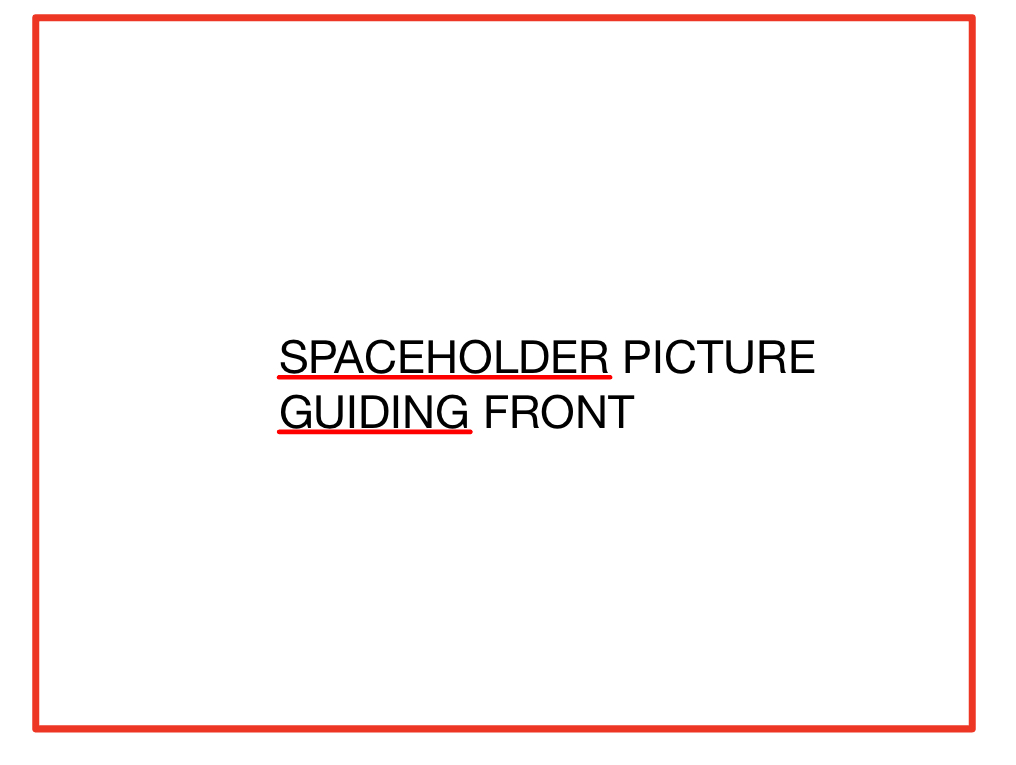
\includegraphics[width=\linewidth]{texfiles/mech/eimg/braking/guiding_front_1.jpg}
    \caption{CAD Guiding Front}
    \label{fig:guiding_front}
  \end{minipage}
  \hspace{0.5cm}
  \begin{minipage}[b]{0.45\linewidth}
    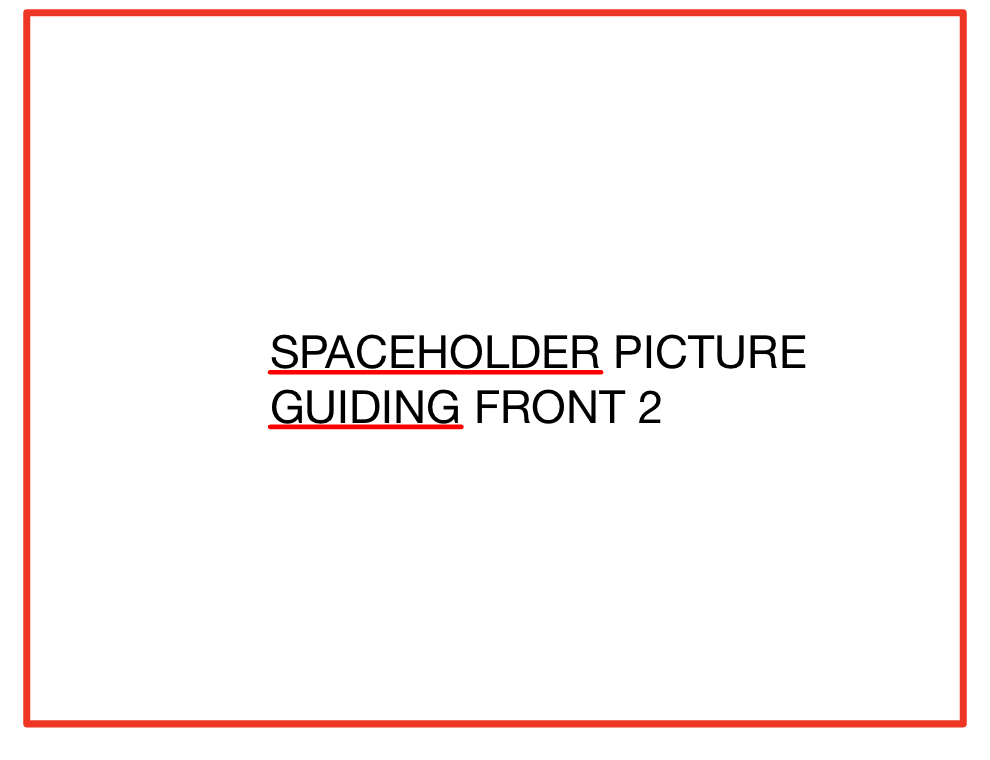
\includegraphics[width=\linewidth]{texfiles/mech/eimg/braking/guiding_front_2.jpg}
    \caption{CAD Guiding Rear}
    \label{fig:guiding_rear}
  \end{minipage}
\end{figure}

\begin{figure}[!ht]
  \centering
  \begin{minipage}[b]{0.45\linewidth}
    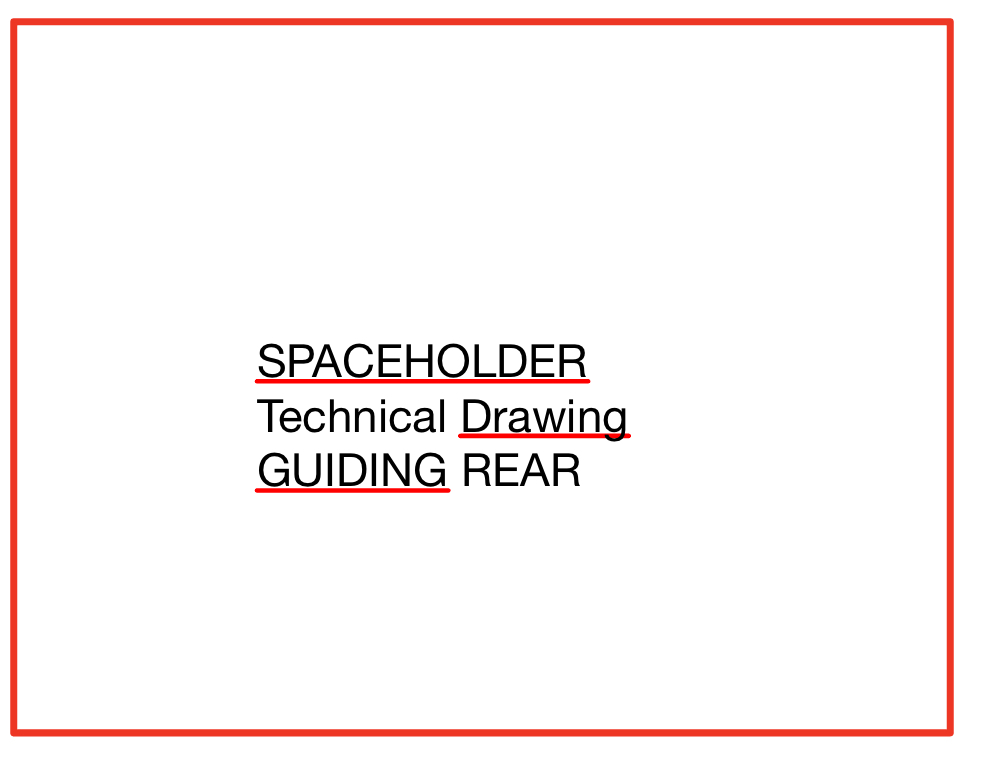
\includegraphics[width=\linewidth]{texfiles/mech/eimg/braking/guiding_tech_rear.jpg}
    \caption{CAD Guiding Front \#2}
    \label{fig:guiding_front_2}
  \end{minipage}
  \hspace{0.5cm}
  \begin{minipage}[b]{0.45\linewidth}
    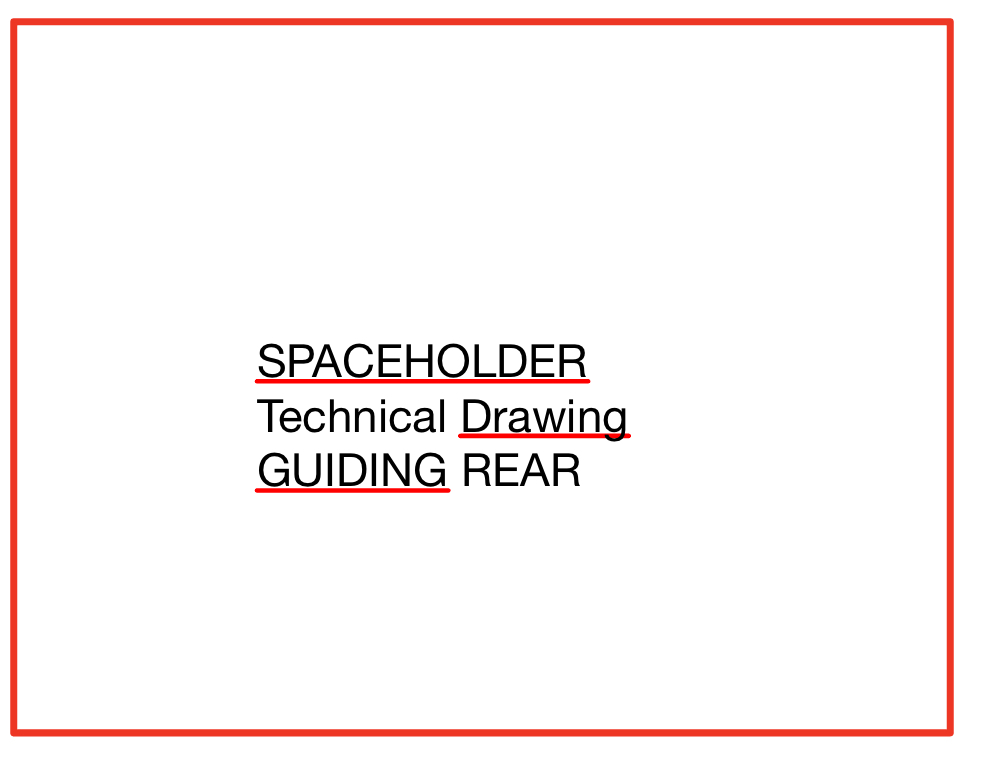
\includegraphics[width=\linewidth]{texfiles/mech/eimg/braking/guiding_tech_rear.jpg}
    \caption{CAD Guiding Rear 2}
    \label{fig:guiding_rear_2}
  \end{minipage}
\end{figure}

\begin{figure}[!ht]
  \centering
  \begin{minipage}[b]{0.45\linewidth}
    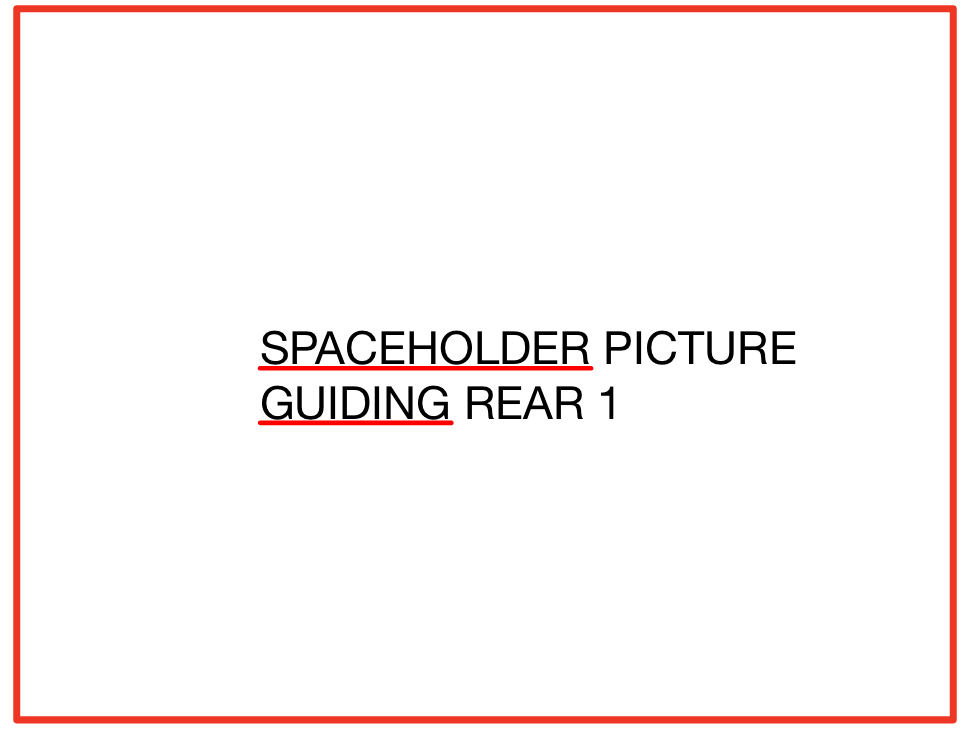
\includegraphics[width=\linewidth]{texfiles/mech/eimg/braking/guiding_rear_1.jpg}
    \caption{Technical Drawing Guiding Front }
    \label{fig:guiding_front_2}
  \end{minipage}
  \hspace{0.5cm}
  \begin{minipage}[b]{0.45\linewidth}
    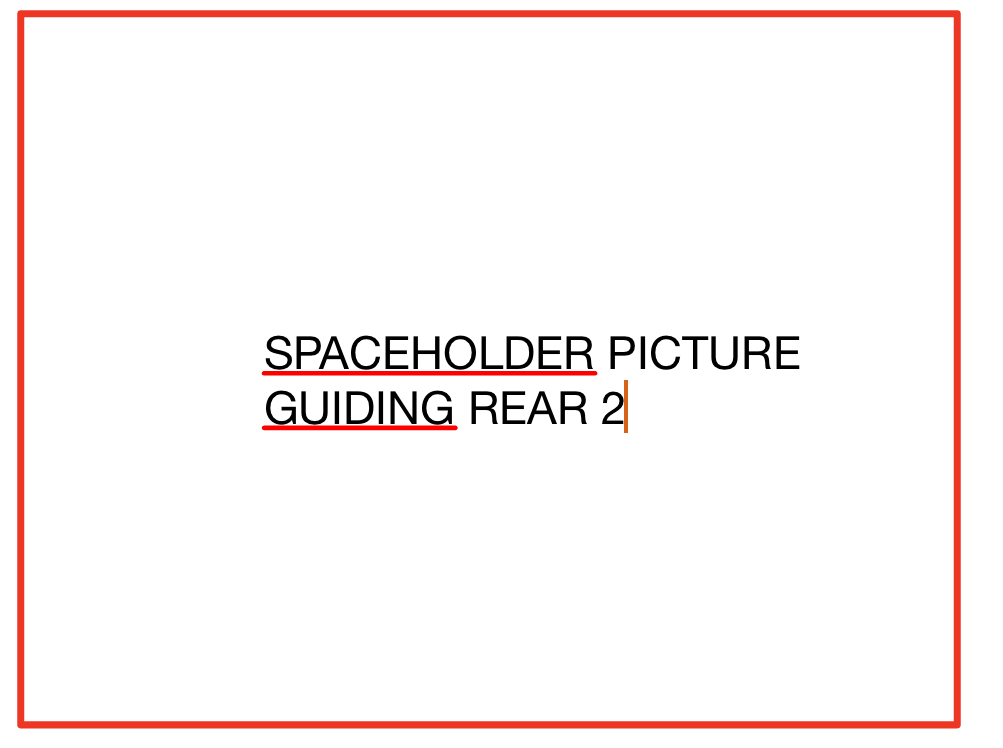
\includegraphics[width=\linewidth]{texfiles/mech/eimg/braking/guiding_rear_2.jpg}
    \caption{Technical Drawing  Guiding Rear}
    \label{fig:guiding_rear_2}
  \end{minipage}
\end{figure}

\newpage
\subsubsection{Materials}
To ensure maximum performance and longevity, the materials used for the subsystem components specifically, the small actuator mounting and the large brake mounting have been carefully chosen.  The choice of plain carbon steel can be attributed to its superior mechanical properties, affordability, and suitability for its intended application. It's also simple to work with and shape during production, which lowers costs and promotes efficient production.


Because plain carbon steel is durable and resistant to corrosion, it can withstand extreme conditions and last for a very long time. It is very easy to weld, which makes assembly simpler.

Finding the ideal mix between strength, the lifespan, ease of manufacture, and cost-effectiveness was the main consideration in the selection of plain carbon steel for these components.

\subsubsection{Design Rationale}
The main goal of the braking system design is to use advanced design ideas and make sure the pod can stop completely within predetermined parameters.

The design's fundamental idea is to use springs to provide a fail-safe mechanism. Our goal in using springs is to create a braking mechanism that can operate even in the case of a leak or system failure. The unique part is how the actuators are used to keep the springs compressed by operating in reverse. This design element strengthens the system's fail-safe capability by guaranteeing that the pod can activate braking even in the event of a malfunction or physical damage.
In conclusion, the braking system's creative use of actuators that operate in reverse and relying on springs are designed to promote safety and dependability. This method guarantees that even in difficult situations, the pod can brake within predefined limits. 
\subsubsection{FEM Results}
.  Present FEM results for worst-case scenarios, including images and values.
\paragraph{\Large{Calculations:}}






\begin{itemize}[leftmargin=*]
    \item[$\bullet$] \textbf{Kinetic Energy}
\end{itemize}

\noindent
For a pod with mass \(m=260\ \text{kg}\) and speed \(v=70\ \text{km/h}\), \textbf{kinetic energy} is defined as
\begin{align*}
    E_k &= \frac{1}{2} mv^2
\end{align*}
Substituting the given values:
\begin{align}
    E_k &= \mathbf{49151} \, \textbf{J}
\end{align}













\begin{itemize}[leftmargin=*]
  \item[\hspace{-1cm}$\bullet$] \textbf{Braking Force}
\end{itemize}
\noindent
To stop the pod within a certain distance, we must account for the work done to compensate for its kinetic energy. According to the principle of work, when an object moves against a force exerted on it, work is done. Specifically, if the object moves through a displacement $d$ while experiencing a constant force $F$, the force performs an amount of work given by




\[
W = F \cdot d
\]

To find the force \( F \) exerted on the pod, given that the work done is \( W = 49151~\text{J} \) and the stopping distance is \( d = 20~\text{m} \), we rearrange the formula:

\begin{align}
F &= \frac{W}{d} \notag \\
\textbf{Braking force } F &= \mathbf{2457.6}\, \textbf{N} 
\end{align}







\begin{itemize}[leftmargin=*]
    \item[$\bullet$] \textbf{Normal Force}
\end{itemize}
\noindent
To determine the required normal force exerted on the brake pads in order to achieve the necessary brake force, consideration must be given to the coefficient of friction ($\mu = 0.36$) between the brake pads and the track surface.






The required normal force (\( N \)) exerted on the brake pads can be calculated using the formula:

\begin{align}
    N &= \frac{F}{\mu} \notag \\     
  \textbf N  &= \mathbf{6826.66} \, \textbf{N}
\end{align}

where \( F = 2457.6 \) and \( \mu = 0.36 \).\\

The normal force per assembly, with consideration for two distinct assemblies, refers to the resultant force exerted perpendicular to the contact surfaces of each respective assembly.\\

\begin{equation}
\textbf{Normal force per assembly} = \mathbf{3413.28 \,N}
\end{equation}

\newpage
\begin{itemize}[leftmargin=*]
    \item[$\bullet$] \textbf{Spring Calculation}
\end{itemize}
\noindent
Given the parameters provided:

\begin{align*}
    \text{Resting length of the spring} (L_0) &= 187 \, \text{mm} \\
    \text{Spring constant} (k) &= 5.97 \, \text{N/mm} \\
    \text{Compressed length of the spring} (L_1) &= 94 \, \text{mm} \\
    \text{Actuator length} (L_{\text{actuator}}) &= 92 \, \text{mm} \\
    \text{Spring used in mounting} (L_{\text{mounting}}) &= 2 \, \text{mm}
\end{align*}
\noindent
When the spring is compressed from its resting length to the compressed length:

\begin{align*}
    \text{Initial Force} (F_{\text{initial}}) &= k \times (L_0 - L_1) \\
    &= 5.97 \times (187 - 94) \, \text{N} \\
    &= 555.21 \, \text{N}
\end{align*}
\noindent
Upon expansion of the spring to accommodate braking, extending to a length of 114 mm:

\begin{align*}
    \text{Force Required} (F_{\text{expansion}}) &= k \times (L_0 - L_{\text{braking}}) \\
    &= 5.97 \times (187 - 114) \, \text{N} \\
    &= 435.81 \, \text{N}
\end{align*}
\noindent
Since each assembly utilizes 8 springs, the total force required for both assemblies is:

\begin{equation}
\begin{aligned}
    \text{Total Force} (F_{\text{total}}) &= \text{Number of springs} \times F_{\text{expansion}}\notag \\
     \end{aligned}
\end{equation}
\begin{equation}
   \mathbf{Total\ Force} = \mathbf{6972.96 \, N}
\end{equation}



Considering the total normal force of 6826.66 N, it appears that the calculated force from the springs exceeds the total normal force, indicating that the system can function properly under these conditions.



\begin{itemize}[leftmargin=*]
    \item[$\bullet$] \textbf{Actuator Force}
\end{itemize}

\noindent
To determine if the chosen actuators can effectively compress and hold the springs to meet the normal force requirement, we need to calculate the total force capacity provided by all actuators. Given that we have 2 big actuators and 4 small actuators, each with a capacity of 686 N (at 6 bar pressure), we can calculate the total force capacity for each assembly:

\[
\textbf{Total force capacity} = \mathbf{4116} \, \textbf{N}
\]

Comparing this with the required normal force of 3413.28 N, we can see that the total force capacity provided by the actuators exceeds the requirement. Therefore, the chosen actuators are sufficient to compress and hold the springs to achieve the desired normal force on the track surface.

\newpage
\begin{itemize}[leftmargin=*]
    \item[$\bullet$] \textbf{Actuator Pressure}
\end{itemize}
\noindent
Given that the system can handle pressures between $6$ to $10$ bar, with $P_1 = 6$ bar and $F_1 = 686$ N (as per the catalogue) where the actuator can exert a force of $686$ N at $6$ bar.\\

With $8$ springs per assembly and a previously calculated compressed spring force of $555.21$ N, the total compressed spring force per assembly is $8 \times 555.21 = 4441.68$ N.\\
\noindent
Utilizing $6$ actuators per assembly, the required force from each actuator is 
\[
F_2 = 740.28 \, \text{N}.
\]

Now, let's calculate the pressure required for the actuators to handle this force: \\
 
- Using the formula $F = P \times A$, where $F_1 = P_1 \times A$ and $F_2 = P_2 \times A$.\\  
\[
P_2 = \frac{P_1 \times F_2}{F_1}.
\]  

- Substituting the given values, 
\begin{equation}
\mathbf{P_2} = \mathbf{6.47} \, \textbf{bar}.
\end{equation}

Hence, the pressure required for the actuators to handle this condition is approximately $6.5$ bar.
\subsubsection{Mesh and Boundary Conditions}
.  Provide details on the type of mesh, boundary conditions, and Free Body Diagrams.


\subsection{Manufacturing Process}
Kindly consult \textbf{Table \ref{table:components}} for reference.\\

\noindent
We've taken steps to ensure that our braking system is more than just a concept and can be manufactured realistically.\\

\noindent
\textbf{Selecting Materials Which Are Easy to Use}: The materials utilized for each component were selected based on their availability and convenience of production for the intended use. for instance, Carbon steel and other common metals, are chosen due to their easy production and wide availability.\\

\noindent
\textbf{Using Standard Parts}: We made an effort to use components that are widely available and simple to assemble, such as tubes, connectors, and adapters. As a result, producers can assemble everything more easily and without the need for specialized tools.\\ 

\noindent
\textbf{Assembly Ease}: The complete brake system's assembly has been taken into consideration. Parts are made to fit together easily, and assembly workers are assisted by clear labelling and instructions when needed.



\subsection{Integration process}
\subsubsection{Assembling}
Bolts will be used to firmly secure the main brake system to the chassis. Then, using specific mounts, small actuators will be fastened to the brake assembly.

Bolts will then be used to secure the aluminium brackets to the actuators. Before pressurizing the system, springs will be positioned between the metal brackets.




\subsubsection{Assembly interaction}
The longitudinal and lateral planes of the chassis must be securely fastened to the main mounting bracket. In in addition to providing structural support to the central section of the chassis, that connection will transmit forces to the chassis, resulting in the creation of a complete system.



\subsection{Safety Considerations}
\subsubsection{Safety Factor}
\textbf{Selecting Strong Materials:} Parts that make up pneumatic brakes, such as brake housings and valves, are made of hard materials such as steel and reinforced rubber These materials can withstand during braking.\\

\noindent
\textbf{To handle pressure safely:} Air brake systems operate under high pressure, so the parts are designed to handle much higher pressures than they will actually experience during normal use This additional capability this ensures that the system remains safe even if pressure fluctuations or screws occur.\\

\noindent
\textbf{Passing safety tests:} All parts in an air brake system go through rigorous tests to ensure they meet safety standards. These tests test things like how well the parts hold up under stress and whether they perform well under different conditions.\\

\noindent
\textbf{Backup system:} Many brake systems have a built-in backup system. For example, if one part fails, there is usually another part that can take over, ensuring that the brakes remain functional in an emergency. In our case, springs are used to create a brake mechanism that can operate even in the event of a leak or system failure. 
\subsubsection{Worst-Case Scenarios}

It can be dangerous to rely solely on air pressure in a standard pneumatic braking system without a fail-safe feature if the pressure drops unexpectedly or if there is a malfunction with the system.  \\

 \noindent
\textbf{Worst case scenario without Fail safe mechanism:}
This system only relies on air pressure. Leak of air or mechanical problem cause the air suddenly disappears, the brake might fail when needed. This makes accidents more likely.\\

\noindent
\textbf{Adding a Fail safe mechanism:}
if there is a problem with air pressure or  in case might be drop, this fail safe feature turns on by itself. it makes sure the brakes keep working even if pressure drop.

\subsection{FMEA Results Discussion}
\subsubsection{Risk Assessment}
.  Preliminary risk assessment for demonstration, transport, and lifting.
\subsubsection{FMEA and Risk Mitigation}
.  Detail FMEA and describe risk mitigation measures.
\subsubsection{Simulation Evidence}
.  Provide evidence of simulations validating theoretical assumptions.


\subsection{Testing}
\subsubsection{Safety Procedures Documentation}
Testing Procedures for Pneumatic Brake System\\

\noindent
\textbf{Pre-Test Inspection:}
Ensuring Braking component are properly attached and free from leaks.\\
Check that the compressed springs are at right place and working properly.\\

\noindent
\textbf{Pressure Check:} With use of pressure gauge to measure the air pressure in the system.\\
Continue increase the pressure to the recommended operating level and check for any pressure drops before operating system.\\

\noindent
\textbf{Monitor the expansion of the spring:}
Verify the expansion of spring as the air pressure decreases.Check that the spring works in Simultaneously with the actuator piston to maintain proper braking force.
Finally, Conduct a final inspection of all components of the system to ensure they remain in good condition.\\

\noindent
\textbf{Activate the Braking system by giving signal:}Check how actuator piston react and check that it moves forward correctly.
verify that the brake pad makes proper contact with the braking surface to create the friction that can enough to slow down the pod.\\

\noindent
\textbf{By applying emergency Brake Test:}
If we have to stop the vehicle in emergency situation,by conducting an emergency brake to check that it can able to quickly stop the pod. 

\subsubsection{Preliminary testing plan}
As we discussed above preliminary testing plan for the pneumatic braking system involves several key tests to validate its functionality and performance.\\
The expected results include regularly pressure build-up, smoother movement of piston, spring expansion and enough friction of brake pad to slow down the vehicle and  Safety precautions will be implemented throughout the testing process to ensure a safe environment and prevent any potential risk.

\subsection{Additional considerations}
\noindent
\subsubsection{Pneumatic Braking System:}
\paragraph{Possible Failures:} Brake systems can malfunction in a number of ways. it include malfunctioning , worn brake pads, pneumatic system failures, air leaks, worn brake pads or discs, electrical issues,  mechanical damage and weather conditions. Regular inspection and maintenance are essential to ensure the system's reliability and safety.
\paragraph{Pressure Requirement:}We are filling the pneumatic system with a pressure of 6.5 bar, well within the system's handling capacity, which ranges between 6 to 10 bar. To ensure that the pressure remains within safe limits, we are using a filling tank and pressure regulator. These components prevent the pressure from exceeding the specified limits and ensure the pneumatic system operates safely and effectively.\\
  
	
\subsection{References}
%Picture of Pneumatic Circuit
